\section{Methodology (Part 1)}

\begin{frame}{Anomaly detection}
\begin{itemize}
  \item \textbf{Anomaly}: Anomalies are data patterns that have vastly
    different characteristics from \textit{normal} data points.
    \item Anomaly detection provides critical and actionable
      information about the data in various domains:
      \begin{itemize}
        \item Anomaly in credit card transactions $\rightarrow$
          Fraudulent use
        \item Anomaly in astronomical images $\rightarrow$
          New celestial body
        \item Anomaly in network traffic $\rightarrow$
          Potential attack
      \end{itemize}
    \item A naive solution: treat this as a (supervised)
      classification problem
    \item This creates a profile for all \textit{`normal'} data points
      and anomalies are those that do not conform to this profile.
    \begin{itemize}
      \item Slower
      \item Lots of false positive
      \item Susceptible to swamping effect
      \item Feasible only in low dimensions
    \end{itemize}
  \item We will \textbf{Isolation Forests} for anomaly detection.
\end{itemize}
\end{frame}
\newpage

% Slide 2
\begin{frame}{Isolation Forest}
\begin{itemize}
    \item Goal: detect anomalies in high-dimensional data
    \item Key idea: anomalies are ``few and different'',
      whereas, \textit{normal} data points are ``many and similar''.
    \item Instead of modeling normal data, we isolate points
    \item Anomalies are those that isolate \textit{easily}.
\end{itemize}
\end{frame}
\newpage

% Slide 3
\begin{frame}{Core Idea}
\begin{itemize}
    \item Build random binary trees called \textbf{isolation trees}
    \item At each node:
    \begin{itemize}
        \item randomly choose a feature
        \item randomly choose a split value
    \end{itemize}
    \item Anomalies tend to be isolated in fewer splits
    \item Normal points require deeper paths to isolate
\end{itemize}
\end{frame}
\newpage

%\begin{frame}{The Isolation Forest Algorithm}

%\end{frame}

\begin{frame}{Scoring Anomalies}
\begin{itemize}
    \item For each point $x$, compute average path length $h(x)$ over trees
    \item Define anomaly score:
    \[
    s(x, n) = 2^{-\frac{h(x)}{c(n)}}
    \]
    where $c(n)$ is average path length in a binary search tree
    \item High score $\Rightarrow$ more anomalous
\end{itemize}
\end{frame}
\newpage

% Slide 5
\begin{frame}{Algorithm Summary}
\begin{enumerate}
    \item Sample subset of data
    \item Build many isolation trees
    \item Compute path lengths for each point
    \item Aggregate to obtain anomaly score
    \item Flag points with high scores as anomalies
\end{enumerate}

\vspace{0.3cm}
\textbf{Key advantage:} No distance or density estimation required
\end{frame}
\newpage

\begin{frame}{The Data}
\justifying{
\begin{itemize}
  \item The data consist of a single JSON file, consisting
    of 3 arrays \footnote{And perhaps some metadata}:
    \begin{itemize}
      \item \texttt{events} \pause
      \item \texttt{entities} \pause
      \item \texttt{relationships} \pause
    \end{itemize}
  \item \texttt{events} is an array consisting of event objects
    which provide the details about the security incidents like
    timestamp, severity score and description. \pause
  \item \texttt{entities} is an array consisting of entity objects
    which provide the details of the affected entity (which could
    be a user, a host, a file, a process \textit{etc.}.) like
    the type of entity and some metadata about them (like name,
    IP address, department etc.). \pause
  \item \texttt{relationships} array gives us the links between
    events and entities and the \textit{`weight'} of the link. \pause
  \item How do we handle this data?
\end{itemize}}
\end{frame}
\newpage

\begin{frame}{Graphs}
\justifying{
\begin{itemize}
  \item A graph $G$ consist of a pair $(V, E)$ of
    vertices $V$ and edges $E \subseteq {V \choose 2}$.
  \item For example, the following graph
    \begin{center}
    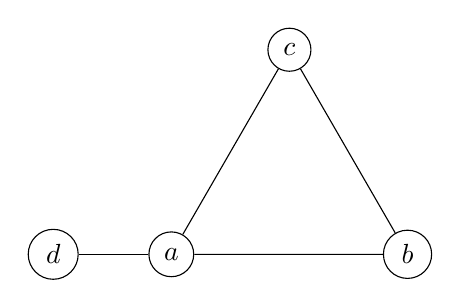
\begin{tikzpicture}[scale=1.5]

    \node[circle,draw] (v1) at (0,0) {$a$};
    \node[circle,draw] (v2) at (2,0) {$b$};
    \node[circle,draw] (v3) at (1,1.732) {$c$};
    \node[circle,draw] (v4) at (-1,0) {$d$};

    \draw (v1) -- (v2) -- (v3) -- (v1);
    \draw (v4) -- (v1);
  \end{tikzpicture}
  \end{center}
  consists of the vertex set $V = \{a, b, c, d\}$
  and the edge set $E = \{\{a, b\}, \{b, c\}, \{c, a\}, \{d, a\}\}$
\end{itemize}}
\end{frame}
\newpage

\begin{frame}{Bipartite Graphs}
\justifying{
\begin{itemize}
  \item  A bipartite graph is a graph whose vertex set $V$
    can be partitioned $G = A \sqcup B$ such that no two vertices
    in $A$ share an edge, and no two vertices in $B$ share an edge.

  \item An example:

    \begin{tikzpicture}[scale=1.2]

% Left part
\node[circle,draw] (u1) at (0,2) {$a_1$};
\node[circle,draw] (u2) at (0,1) {$a_2$};
\node[circle,draw] (u3) at (0,0) {$a_3$};

% Right part
\node[circle,draw] (v1) at (3,2) {$b_1$};
\node[circle,draw] (v2) at (3,1) {$b_2$};
\node[circle,draw] (v3) at (3,0) {$b_3$};

% Labels for the bipartition
\node[left=1cm of u2] {$A$};
\node[right=1cm of v2] {$B$};

% Edges
\draw (u1) -- (v1);
\draw (u1) -- (v2);
\draw (u2) -- (v2);
\draw (u2) -- (v3);
\draw (u3) -- (v1);

\end{tikzpicture} \pause

\item What is a criterion to determine if a graph is bipartite? \pause
\item No odd cycle $\iff$ Bipartite

\end{itemize}}
\end{frame}
\newpage

\begin{frame}{How to handle the data?}
\justifying{
\begin{itemize}
  \item We build a bipartite graph out of the provided data as follows: \pause
  \item We let the vertex set be \texttt{events} $\sqcup$ \texttt{entities}. \pause
  \item We let the edge set be the \texttt{relationships}. \pause
  \item An example:
    \begin{center}
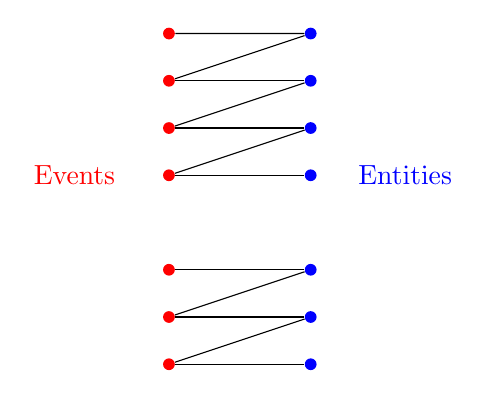
\begin{tikzpicture}[scale=0.6,
    every node/.style={circle,fill,inner sep=1.5pt}]

% Partition labels
\node[draw=none,fill=none, color=red] at (-2,2) {Events};
\node[draw=none,fill=none, color=blue] at (5,2) {Entities};

%========================
% Component 1 (4+4)
%========================

% A-side
\node[color=red] (a1) at (0,5) {};
\node[color=red] (a2) at (0,4) {};
\node[color=red] (a3) at (0,3) {};
\node[color=red] (a4) at (0,2) {};

% B-side
\node[color=blue] (b1) at (3,5) {};
\node[color=blue] (b2) at (3,4) {};
\node[color=blue] (b3) at (3,3) {};
\node[color=blue] (b4) at (3,2) {};

% Edges
\draw (a1)--(b1);
\draw (a2)--(b1);
\draw (a2)--(b2);
\draw (a3)--(b2);
\draw (a3)--(b3);
\draw (a4)--(b3);
\draw (a4)--(b4);

%========================
% Component 2 (3+3)
%========================

% A-side
\node[color=red] (c1) at (0,0) {};
\node[color=red] (c2) at (0,-1) {};
\node[color=red] (c3) at (0,-2) {};

% B-side
\node[color=blue] (d1) at (3,0) {};
\node[color=blue] (d2) at (3,-1) {};
\node[color=blue] (d3) at (3,-2) {};

% Edges
\draw (c1)--(d1);
\draw (c2)--(d1);
\draw (c2)--(d2);
\draw (c3)--(d2);
\draw (c3)--(d3);

\end{tikzpicture}
\end{center}
\pause
\item Observe that this example has 2 connected components.
\end{itemize}}
\end{frame}
\newpage

\begin{frame}{Isolating the anomalous components}
  \justifying{
  \begin{itemize}
    \item We feed the connected components of this graph
      to the isolation forest algorithm.
    \item The pipeline: \begin{center}
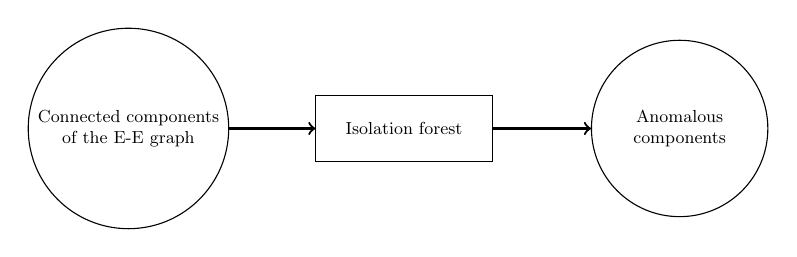
\begin{tikzpicture}[
    scale=0.7,
    transform shape,
    node distance=5cm,
    every node/.style={font=\small},
    circ/.style={circle,draw,minimum width=3.2cm,align=center},
    box/.style={rectangle,draw,minimum width=3.2cm,minimum height=1.2cm,align=center}
]

\node[circ] (start) {Connected components\\of the E-E graph};

\node[box,right of=start] (iso) {Isolation forest};

\node[circ,right of=iso] (end) {Anomalous\\components};

\draw[->,thick] (start) -- (iso);
\draw[->,thick] (iso) -- (end);

\end{tikzpicture}


      \end{center}
    \item The components with high anomaly score are likely
      to be attack scenarios.
  \end{itemize}}
\end{frame}
\newpage

\begin{frame}
  \begin{itemize}
    \item In practice, most hash functions use some kind of
      mixing algorithm that transforms string of length
      $n$ into another string of length $n$.
    \item The hash function breaks the string into blocks
      of length $n$.
    \item $m = m_1 || m_2 || \dots || m_k$.
    \item Then it combines iteratively combines each block
      with the previously computed hash value using the
      mixing algorithm.
  \end{itemize}
\end{frame}
